\documentclass[letter,12pt]{article}
\usepackage{graphicx}
\usepackage{url}
\usepackage{setspace}
\usepackage{ragged2e}
\usepackage{hanging}
\usepackage{hyperref}
\usepackage{fancyhdr}
\usepackage{lipsum}
\usepackage[none]{hyphenat}
\usepackage{enumitem}
\usepackage{amsmath}
\usepackage{parskip}
\usepackage{indentfirst}

\makeatletter
\newcommand{\distas}[1]{\mathbin{\overset{#1}{\kern\z@\sim}}}
\newsavebox{\mybox}\newsavebox{\mysim}
\newcommand{\distras}[1]{%
	\savebox{\mybox}{\hbox{\kern3pt$\scriptstyle#1$\kern3pt}}%
	\savebox{\mysim}{\hbox{$\sim$}}%
	\mathbin{\overset{#1}{\kern\z@\resizebox{\wd\mybox}{\ht\mysim}{$\sim$}}}%
}
\makeatother

\fancyhead{}
\fancyhead[L]{PREDICTING DIABETES}
\fancyhead[R]{\thepage}
\fancyfoot{}
\fancypagestyle{plain}{
	\fancyhead{}
	\fancyhead[L]{Running head: PREDICTING DIABETES}
	\fancyfoot{}
	\fancyhead[R]{\thepage}
}
\pagestyle{fancy}
\renewcommand{\headrulewidth}{0pt}
\addtolength{\headwidth}{\marginparsep}
\addtolength{\headwidth}{\marginparwidth}

\doublespacing

\addtolength{\oddsidemargin}{-.5in}
\addtolength{\evensidemargin}{-.5in}
\addtolength{\textwidth}{1in}

\addtolength{\topmargin}{-.875in}
\addtolength{\textheight}{1.75in}

\begin{document}
	\thispagestyle{plain}
	\begin{center}
		\vspace*{150pt}
		Predicting Contributing Factors to Diabetes. \\
		Sejin Kim \\
		Kenyon College \\
	\end{center}
	\vspace*{120pt}
	\centering{Author Note} \\
	\begin{raggedright}
		Sejin Kim, Kenyon College. \\
		Contact: \href{mailto:kim3@kenyon.edu}{kim3@kenyon.edu} \\
		\vspace*{40pt}
		\textit{Keywords:} diabetes, nhanes, regression
	\end{raggedright}
	
	\newpage

	\begin{center}
		Predicting Contributing Factors to Diabetes.
	\end{center}
	\begin{center}
		\textbf{I. Introduction}
	\end{center}
	\justify
	\indent Diabetes has long plagued the world, but within the past 60 years, the number of people affected by this disease has increased dramatically. The CDC estimated that in 2015, just under 8\% of the United States population was diagnosed with diabetes. According to a brief time series analysis of the historical data that the CDC publishes from 1980 to 2017, the rate of diabetes is continuing to grow. An ACF plot found that at four lags in, the present values for the total percentage of the population with diabetes is well related with the past total percentage reports. If we are to continue on this path, we could see changes within the healthcare and pharmaceutical industries that may not be for the best.\par
	To further explore this, we are using a dataset from the National Health and Nutrition Examination Survey. The "survey" is actually a group of surveys, each designed to "assess the health..of adults and childre in the United States." While some surveys are very much qualitative information, the data that we will be analyzing is purely quantitative.\par
	The NHANES program began in the 1960's, and is a major program section at the Centers for Disease Control and Prevention. It is used by both government and institutional analysts to find patterns in the approaches to and general sentiment towards healthcare and nutrition domestically. Because of its comprehensive nature, it is widely applicable for modeling and predicting patterns in many diifferent fields. The data has been used to create growth charts for children, develop the policy to remove lead from common household items, influence immunization schedules, and track diabetes. All of the data is collected and anonymized to protect the healthcare rights afforded by HIPPA. \par
	While some of this data can be used in isolation, say to determine the rates of change in diabetes diagnoses, more comprehensive data can be used to holistically determine if there are leading causes in diabetes, including changes which may not have been foreseen at the beginning of the data collection, but which is due to more than just chance.\par
	The NHANES dataset were retrieved in a cleaned form from the Kenyon College department of statistics. The dataset originally included about 10,000 observations across 70 different variables. The applicable dataset was cleaned to only include 2167 observations across 28 different variables. The data includes observations gathered from 2009 to 2012's biannual surveys, and the dataset was filled on a rolling schedule.\par
	

	\begin{center}
		\textbf{III. Methods}
	\end{center}
	\justify
	%Text goes here
	Analysis began by exploring the data graphically. To determine if there were any variables that were heavily correlated with each other, a numerical correlation matrix and the accompanying $p$-value matrix were created. In analyzing this correlation matrix, I tagged correlations which had a correlation $cor > 0.25$ and $p > 0.05 = \alpha$ to find if any of these variables were heavily correlated with each other, and whether those correlations were due to more than just chance. Given a dataset with this many variables, some overlap and high correlations between variables is to be expected.\par
	The correlations that were found did make sense. The variable \textit{HomeRooms} was correlated to \textit{HHIncomeMid}, which makes sense because as income increases, the number of rooms in your home would also increase. \textit{Height}, \textit{Weight}, and \textit{BMI} are all highly correlated, which makes sense, since BMI is derived from both height and weight, by the CDC's definition\footnote{Of note is that the CDC does NOT take into account the gender, but different BMI models may take this into account. For the purposes of this study, gender is not used.}. As expected, average diastolic blood pressure (\textit{BPDiaAve}) and average systolic blood pressure (\textit{BPSysAve}) are also related. Of note is that only the average systolic blood pressure is somewhat highly correlated with age, not average diastolic blood pressure. Finally, the first urine flow rate measurement (\textit{UrineFlow1}) is somewhat highly correlated with the volume of urine (\textit{UrineVol1}). There were no other variables which had a high correlation that were also significant.
	Plots were made for most of the variables, against the binary variable \textit{Diabetes}. The expected behavior here was that for any given boxplot, the majority of every group would be within the box, which should have been clustered around 0. Some groups may have had an outlier of diabetics, if the variable were to be significant or heavily correlated, which would show up in any boxplot as a group of outlier points where \textit{Diabetes} = 1. Several of these plots are given as follows.
	\begin{center}
	  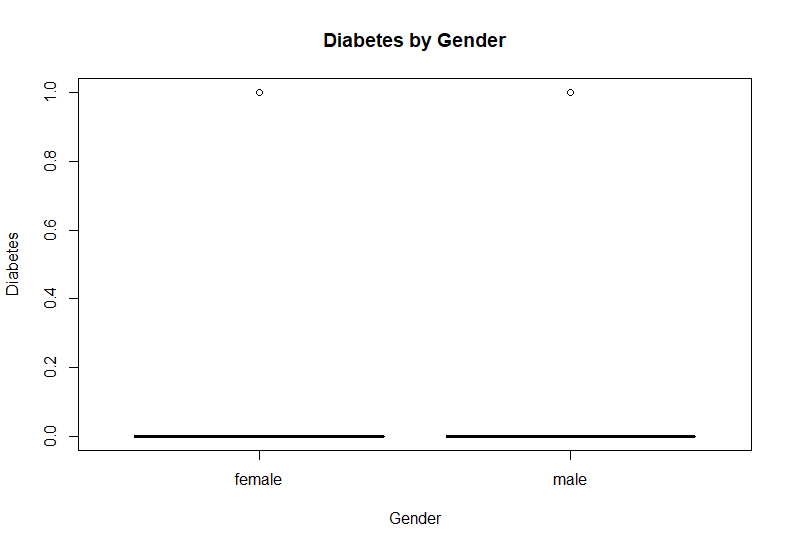
\includegraphics[width=0.6\textwidth]{img/boxdiabetesgender.png}
	  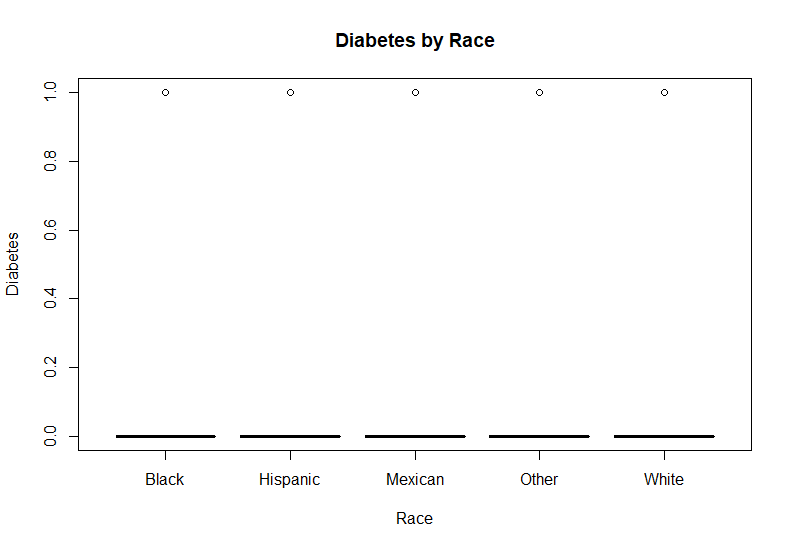
\includegraphics[width=0.6\textwidth]{img/boxdiabetesrace.png}
	  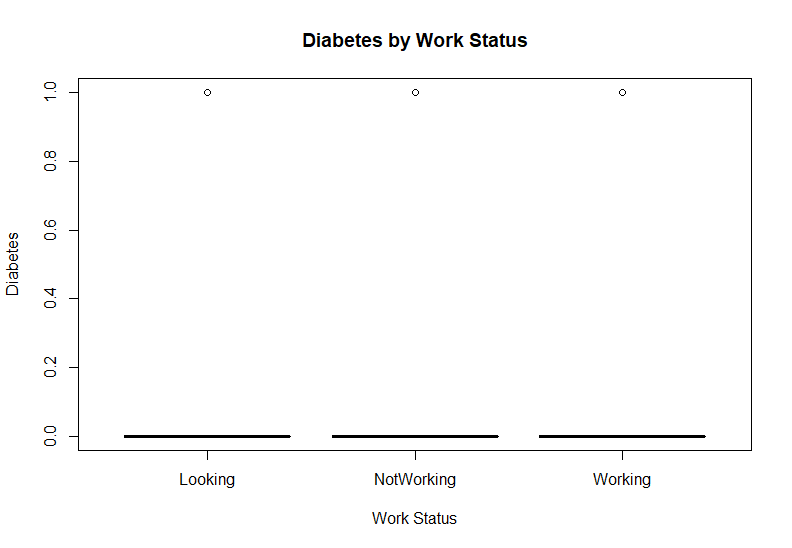
\includegraphics[width=0.6\textwidth]{img/boxdiabeteswork.png}
	  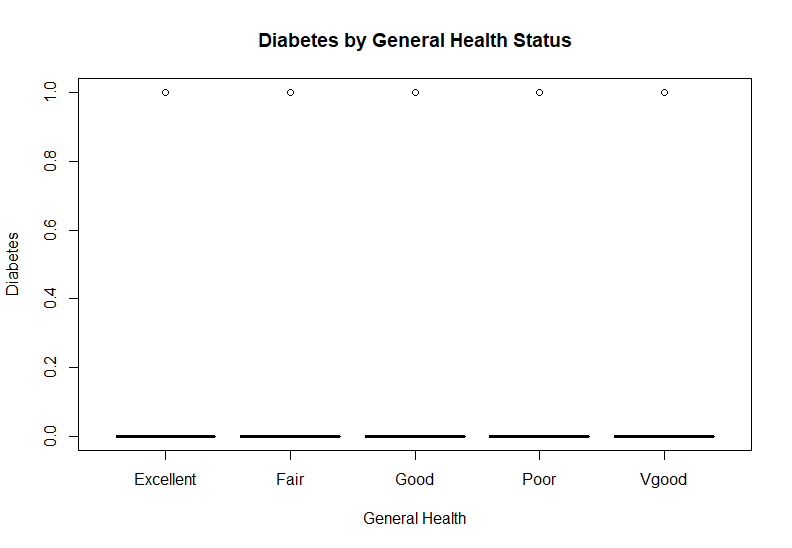
\includegraphics[width=0.6\textwidth]{img/boxdiabeteshealthgen.png}
	\end{center}
	As shown, the behavior of each of these plots is to be expected. The majority of the surveyed individuals do not have diabetes. This is backed up with summary statistics, which report that only 145 out of the 2167 observations report having diabetes.\par
	The multiple logistic regression models were determined using a stepwise procedure using the \verb|step| function in R. This function selects models to minimize the AIC value, rather than by only using the smallest $p$-value. Like any model building procedure, including those for linear regression model building, one should not blindly accept the results based on the output from the computer, but rather should double check the model or build a second model from available variabls that are biologically or scientifically sensible. That is, it would not make sense for the observation number to be a significant variable. If it were to show up significantly (it does not, but for the sake of this example, let us continue to use it), we should strongly consider throwing it out, since it is an artificial variable that only affects the regression by chance.\par
	In this analysis, we will be using multiple correlation to investigate the relationship between potential independent variables. For example, if two independent variables have some uncanny relationship to one another, we will likely drop at least one of them in the final model, which ever one is less significant. There may be reasons why we would choose one variable over another one for the final model, though. In this dataset, let us examine the \textit{BMI} variable. According to the CDC, BMI is derived from height and from weight, both of which are supposedly independent variables. As a result, in our final analysis, we probably would \textit{not} want to use all three of these variables, but rather which ever variable accounts for the most variability.\par
	After creating the initial model using stepwise logistic regression, the model was examined more closely to check for abnormal behavior, especially in the z-values and the $p$-values. In the initial model generated by the stepwise regression method, the average systolic blood pressure showed itself to not be a significant and meaningful variable in the regression. As a result, I chose to remove it from the regression. To ensure that the change to the model was truly appropriate, I also examined the Wald statistics using the type II tests in ANOVA, and found that the $p$-value, the probability that the average systolic blood pressure was in the model due to more than just chance, was above my model's cutoff value of $\alpha = 0.1$.\par
	Through this analysis, the final model is as follows:
	\begin{equation}
	\begin{split}
  	log(Odds) = \beta_{0} + \beta_{1} \times (Age) + \\\beta_{2} \times (BMI) + \\\beta_{3} \times (TotChol) + \\\beta_{4} \times (DaysPhysHlthBad) + \\\beta_{5} \times (HealthGen(Fair)) + \\\beta_{6} \times (HealthGen(Good)) + \\\beta_{7} \times UrineVol1 + \\\beta_{8} \times (DirectChol) + \\\beta_{9} \times (DaysMentHlthBad) + \\\beta_{10} \times (Work(NotWorking)) + \epsilon \distas{iid} N(0,\sigma)
	\end{split}
	\end{equation}
	When we fit this model to the data, we get the following logistic regression line for the data:
	\begin{equation}
	\begin{split}
  	\hat{log(Odds)} = -5.350001 + 0.077244 \times (Age) + \\ 0.078084 \times (BMI) - \\ 0.442099 \times (TotChol) + \\ 0.045104 \times (DaysPhysHlthBad) + \\ 1.236488 \times (HealthGen(Fair)) + \\ 0.658304 \times (HealthGen(Good)) - \\ 0.003053 \times UrineVol1 - \\ 0.611166 \times (DirectChol) - \\ 0.034084 \times (DaysMentHlthBad) - \\ 1.040257 \times (Work(NotWorking)) + \epsilon \distas{iid} N(0,\sigma)
	\end{split}
	\end{equation}
	To continue my analysis, I also generated an overall $p$-value for the model. To do this, I defined the null model and compared it to the full model using an analysis of variance, or ANOVA. I used the $\chi^{2}$ distribution to run this test. In this test, I found that with a residual deviance of 1111.18 on 2166 degrees of freedom and a $p$-value of $\approx 0$ (reported as $2.2 \times 10^{-16}$, we reject the null hypothesis that the final model generated is significantly different from the null model. In the same vein as the ANOVA, I also ran a likelyhood ratio test of nested models. In this analysis, I found that with a log-likelyhood of -555.59 on one degree of freedom, and a $p$-value of $\approx 0$ (reported as $2.2 \times 10^{-16}$, we reject the null hypothesis that the models are similar. The primary difference between this test and the ANOVA from above is that this test is an asymptotic likelyhood test, and uses the Wald test as its base.\par

	\begin{center}
		\textbf{III. Results}\par
	\end{center}
	\justify
	%Text goes here
	
	
	\begin{center}
		\textbf{V. Conclusion}\par
	\end{center}
	\justify
  %Text goes here
	
	\newpage
	
	\begin{center}
		Works Cited
	\end{center}
	\raggedright
	\begin{hangparas}{.5in}{1}
		Felipe de Mendiburu (2019). agricolae: Statistical Procedures for Agricultural Research. R package version 1.3-1. https://CRAN.R-project.org/package=agricolae
	\end{hangparas}
	\begin{hangparas}{.5in}{1}
	  Frank E Harrell Jr, with contributions from Charles Dupont and many others. (2019). Hmisc: Harrell Miscellaneous. R package version 4.2-0. https://CRAN.R-project.org/package=Hmisc
	\end{hangparas}
	\begin{hangparas}{.5in}{1}
		John Fox and Sanford Weisberg (2019). An {R} Companion to Applied Regression, Third Edition. Thousand Oaks CA: Sage. URL: https://socialsciences.mcmaster.ca/jfox/Books/Companion/
	\end{hangparas}
	\begin{hangparas}{.5in}{1}
	  Max Kuhn. Contributions from Jed Wing, Steve Weston, Andre Williams, Chris Keefer, Allan Engelhardt, Tony Cooper, Zachary Mayer, Brenton Kenkel, the R Core Team, Michael Benesty, Reynald Lescarbeau, Andrew Ziem, Luca Scrucca, Yuan Tang, Can Candan and Tyler Hunt. (2019). caret: Classification and Regression Training. R package version 6.0-84. https://CRAN.R-project.org/package=caret
	\end{hangparas}
	\begin{hangparas}{.5in}{1}
		R Core Team (2019). R: A language and environment for statistical computing. R Foundation for Statistical Computing, Vienna, Austria. URL https://www.R-project.org/.
	\end{hangparas}
	\begin{hangparas}{.5in}{1}
		R. Pruim, D. T. Kaplan and N. J. Horton. The mosaic Package: Helping Students to 'Think with Data' Using R (2017). The R Journal, 9(1):77-102.
	\end{hangparas}
	\begin{hangparas}{.5in}{1}
	  Richard M. Heiberger (2019). HH: Statistical Analysis and Data Display: Heiberger and Holland. R package version 3.1-37. URL https://CRAN.R-project.org/package=HH
	\end{hangparas}
	\begin{hangparas}{.5in}{1}
		Stephane Champely (2018). pwr: Basic Functions for Power Analysis. R package version 1.2-2. https://CRAN.R-project.org/package=pwr
	\end{hangparas}
	\begin{hangparas}{.5in}{1}
	  Thomas Lumley based on Fortran code by Alan Miller (2017). leaps: Regression Subset Selection. R package version 3.0. https://CRAN.R-project.org/package=leaps
	\end{hangparas}
	\begin{hangparas}{.5in}{1}
		Torsten Hothorn, Frank Bretz and Peter Westfall (2008). Simultaneous Inference in General Parametric Models. Biometrical Journal 50(3), 346--363.
	\end{hangparas}
	\begin{hangparas}{.5in}{1}
	  U.S. Department of Health and Human Services. (2017). National Health and Nutrition Examination Survey. National Center for Health Statistics, Centers for Disease Control and Prevention.
	\end{hangparas}
	\begin{hangparas}{.5in}{1}
	  U.S. Department of Health and Human Services. (2017). Diagnosed Diabetes. Division of Diabetes Translation, United States Diabetes Surveillance System, Centers for Disease Control and Prevention.
	\end{hangparas}
\end{document}
